\documentclass{ximera}

\usepackage{float}

\newcommand{\R}{\mathbb R}

\newcommand{\href}[2]{#2\footnote{\url{#1}}}
\newcommand{\verticalvector}[1]{\begin{bmatrix}#1\end{bmatrix}}
\newcommand{\gt}{>}

\pgfplotsset{compat=1.8}
\graphicspath{
{./}
{introduction/}
{unit1/}
{unit1/theGeometryOfLinearEquations/}
{unit1/EliminationwithMatrices/}
{unit1/MultiplicationandInverseMatrices/}
}


\title{Elimination with matrices}

\begin{document}
\begin{abstract}
  Unit 1 MIT OCW Linear Algebra: Elimination with matrices
\end{abstract}
\maketitle

The MIT OCW Video Lecture can be found
here:\video{https://www.youtube.com/watch?v=QVKj3LADCnA}

This session introduces the method of elimination, an essential tool for working 
with matrices. The method follows a simple algorithm. To help make sense of material 
presented later, we describe this algorithm in terms of matrix multiplication.

\begin{figure}[H]
\begin{image}
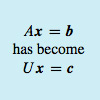
\includegraphics{1_2.jpg}
\end{image}
\end{figure}

\section*{Method of Elimination}

\[A = \begin{bmatrix} 1&2&1\\3&8&1\\0&4&1 \end{bmatrix}\]and\[\mathbf{b} = \verticalvector{2\\12\\2}\]


The number $1$ in the upper left corner of $A$ is called the first pivot. We 
recopy the first row, then multiply the numbers in it by an appropriate value 
(in this case $3$) and subtract those values from the numbers in the second row.
The first number in the second row becomes $0$. We have thus eliminated the $3$ 
in row $2$ column $1$.

The next step is to perform another elimination to get a $0$ in row $3$ column $1$; 
here this is already the case.

The second pivot is the value $2$ which now appears in row $2$ column $2$. 
We find a multiplier (in this case $2$) by which we multiply the second row to 
eliminate the $4$ in row $3$ column $2$. The third pivot is then the $5$ 
now in row $3$ column $3$.

We started with an invertible matrix $A$ and ended with an upper triangular matrix $U$;
the lower left portion of U is filled with zeros. Pivots 1, 2, 5 are on the diagonal
of $U$.

\[A = \begin{bmatrix} 1&2&1\\3&8&1\\0&4&1 \end{bmatrix} \longrightarrow
\begin{bmatrix} 1&2&\phantom{-} 1\\0&2&-2\\0&4&\phantom{-} 1 \end{bmatrix} 
\longrightarrow U = \begin{bmatrix} 1&2&\phantom{-}1\\0&2&-2\\0&0&\phantom{-}5 \end{bmatrix} 
\]

We repeat the multiplications and subtractions with the vector $B = \verticalvector{2\\12\\2}$

For example, we multiply the $2$ in the first position by $3$ and subtract from $12$
to get $6$ in the second position. When calculating by hand we can do this efficiently
by augmenting the matrix $A$, appending the vector $b$ as a fourth or final column. 
The method of elimination transforms the equation $A\mathbf{x} = \mathbf{b}$ 
into a new equation $U\mathbf{x} = \mathbf{c}$. In the example above 
$U = \begin{bmatrix} 1&2&\phantom{-}1\\0&2&-2\\0&0&\phantom{-}5 \end{bmatrix}$
comes from $A$ and $c=\verticalvector{\phantom{-}2\\\phantom{-}6\\-10}$ comes from 
$\mathbf{b}$.

The equation $U\mathbf{x} = \mathbf{c}$ is easy to solve by back substitution; 
in our example, $z = -2$, $y = 1$ and $x = 2$. This is also a solution to the 
original system $A\mathbf{x} = \mathbf{b}$.

The determinant of $U$ is the product of the pivots. We will see this again.

Pivots may not be $0$. If there is a zero in the pivot position, we must exchange 
that row with one below to get a non-zero value in the pivot position. 

If there is a zero in the pivot position and no non-zero value below it, 
then the matrix $A$ is not invertible. Elimination can not be used to find a 
unique solution to the system of equations as it doesnt exist.

\section*{Elimination Matrices}

The product of a matrix $(3x3)$ and a column vector $(3x1)$ is a column vector 
$(3x1)$ that is a linear combination of the columns of the matrix.

The product of a row $(1x3)$ and a matrix $(3x3)$ is a row $(1x3)$ that is a linear
combination of the rows of the matrix.

We can subtract $3$ times row $1$ of matrix $A$ from row $2$ of $A$ by calculating 
the matrix product:

\[
\begin{bmatrix} \phantom{-}1&0&0\\-3&1&0\\\phantom{-}0&0&1 \end{bmatrix}
\cdot 
\begin{bmatrix} 1&2&1\\3&8&1\\0&4&1 \end{bmatrix} =
\begin{bmatrix} 1&2&\phantom{-}1\\0&2&-2\\0&4&\phantom{-}1 \end{bmatrix}
\]

The elimination matrix used to eliminate the entry in row m column n is denoted $E_{mn}$. 
The calculation above took us from $A$ to $E_{21}A$. The three elimination steps 
leading to $U$ were: $E_{32}(E_{31}(E_{21}A)) = U$, where $E_{31} = I$. Thus 
$E_{32}(E_{21}A) = U$.

Matrix multiplication is associative, so we can also write $(E_{32}E_{21})A = U$. 
The product $E_{32}E_{21}$ tells us how to get from $A$ to $U$. The inverse of the matrix 
$E_{32}E_{21}$ tells us how to get from $U$ to $A$.

If we solve $U\mathbf{x} = EA\mathbf{x} = E\mathbf{b}$, then it is also true that 
$A\mathbf{x} = \mathbf{b}$. This is why the method of elimination works: all steps 
can be reversed.

A permutation matrix exchanges two rows of a matrix; for example,

\[
P=\begin{bmatrix} 0&1&0\\1&0&0\\0&0&1 \end{bmatrix}
\]

The first and second rows of the matrix $PA$ are the second and first rows of the 
matrix $A$. The matrix $P$ is constructed by exchanging rows of the identity matrix.

To exchange the columns of a matrix, multiply on the right (as in $AP$) by a 
permutation matrix.

Note that matrix multiplication is not commutative: $PA \neq AP$.

\section*{Inverses}

We have a matrix:

\[
 E_{21} = \begin{bmatrix} \phantom{-}0&1&0\\-3&1&0\\\phantom{-}0&0&1 \end{bmatrix}
\]

which subtracts 3 times row 1 from row 2. To undo this operation we must add 3 times 
row 1 to row 2 using the inverse matrix:

\[
 E_{21}^{-1} = \begin{bmatrix} 0&1&0\\3&1&0\\0&0&1 \end{bmatrix}
\]


In fact, $ E_{21}^{-1}E_{21} = I$.


\begin{question}
\begin{solution}
\begin{hint}
\end{hint}
The answer is \answer{true}
\end{solution}
\end{question}

\end{document}
